\documentclass[11pt,a4paper]{article}
\usepackage[catalan]{babel}

% Paquetes necesarios
% preamble.tex

% Codificación y tipografía
\usepackage[utf8]{inputenc}
\usepackage[T1]{fontenc}
\usepackage[catalan]{babel}
\usepackage{lmodern}

% Márgenes y geometría
\usepackage{geometry}
\geometry{left=2.5cm, right=2.5cm, top=2cm, bottom=3cm}
% Estilo de página
\usepackage{fancyhdr}
\setlength{\headheight}{15pt}
\pagestyle{fancy}
\fancyhf{}
\lhead{\textit{Electrònica Física}}
\rhead{\textit{Adrià Rojo}}
\cfoot{\thepage}

% Gráficos y tablas
\usepackage{graphicx}
\usepackage{float}
\usepackage{caption}

% Matemáticas y símbolos
\usepackage{amsmath}
\usepackage{amssymb}

% Hipervínculos
\usepackage{hyperref}

% Espaciado
\usepackage{parskip}  % Quita sangría de párrafos y añade espacio
\usepackage{wrapfig}
\usepackage[backend=biber,style=ieee, autocite=superscript]{biblatex}
\addbibresource{bibliography.bib}

% Fuente y estilo general
\renewcommand{\familydefault}{\rmdefault}

%Definició de la ela geminada per tal que accepti el punt volat del teclat
% \def·#1{%
%   \ifmmode
%     \cdot #1
%     %\csname normal@char\string"\endcsname l%
%   \else%
%     \def\argument{#1}%
%     \if\argument l%
%       \leftllkern=0pt\rightllkern=0pt\raiselldim=0pt%
%       \setbox0\hbox{l}\setbox1\hbox{l\/}\setbox2\hbox{.}%
%       \advance\raiselldim by \the\fontdimen5\the\font
%       \advance\raiselldim by -\ht2%
%       \leftllkern=-.25\wd0%
%       \advance\leftllkern by \wd1%
%       \advance\leftllkern by -\wd0%
%       \rightllkern=-.25\wd0%
%       \advance\rightllkern by -\wd1%
%       \advance\rightllkern by \wd0%
%       \allowhyphens\discretionary{-}{l}%
%       {\hbox{}\kern\leftllkern\raise\raiselldim\hbox{.}%
%         \kern\rightllkern\hbox{l}}\allowhyphens%
%     \else
%       \if\argument L%
%         \leftllkern=0pt\rightllkern=0pt\raiselldim=0pt%
%         \setbox0\hbox{L}\setbox1\hbox{L\/}\setbox2\hbox{.}%
%         \advance\raiselldim by .5\ht0%
%         \advance\raiselldim by -.5\ht2%
%         \leftllkern=-.125\wd0%
%         \advance\leftllkern by \wd1%
%         \advance\leftllkern by -\wd0%
%         \rightllkern=-\wd0%
%         \divide\rightllkern by 6%
%         \advance\rightllkern by -\wd1%
%         \advance\rightllkern by \wd0%
%         \allowhyphens\discretionary{-}{L}%
%         {\hbox{}\kern\leftllkern\raise\raiselldim\hbox{.}%
%            \kern\rightllkern\hbox{L}}\allowhyphens%
%       \else
%         #1
%       \fi
%     \fi
%   \fi
%   }
% Título
\title{\textbf{CMOS: Història, fonaments i funcionament i aplicacions}}
\author{Adrià Rojo}
\date{\today}

\begin{document}

\maketitle
\thispagestyle{empty}
% Resumen
\begin{abstract}
    BLABLA
\end{abstract}

\section{Introducció}
% Introducir brevemente qué es CMOS, su importancia en la electrónica digital y qué estructura tendrá el trabajo.

Un semiconductor-òxid-metall complementari (\textit{Complementary-Metal-Oxide Semiconductor}) o CMOS, és un tipus de tecnologia que combina un parell simètric de NMOS i PMOS connectats de forma complementària per poder fer operacions lògiques de forma eficient\autocite{wiki:CMOS}. 

Aquesta tecnologia és la base d'electrònica moderna, sent el bloc principal de la porta lògica \texttt{NAND}, que és la base de tots els altres circuits existents i pot arribar formar circuits molt complexos com processadors i memòries RAM.

Els dispositius dissenyats amb el procés CMOS en ment també poden ser utilitzats com a sensor d'imatge, gràcies a la seva eficiència i rapidesa, formant part d'una àmplia varietat d'eines electròniques, des de telèfons mòbils a drons i càmeres fotogràfiques utilitzades en medicina o astronomia. 

Actualment s'estima que el nombre de transistors MOSFET manufacturats (inclou els CMOS) superen els $10^{22}$ dispositius \autocite{wiki:Transistor_count} al 2018, dada que està basada en la Llei de Moore.

\begin{figure}[h]
    \centering
    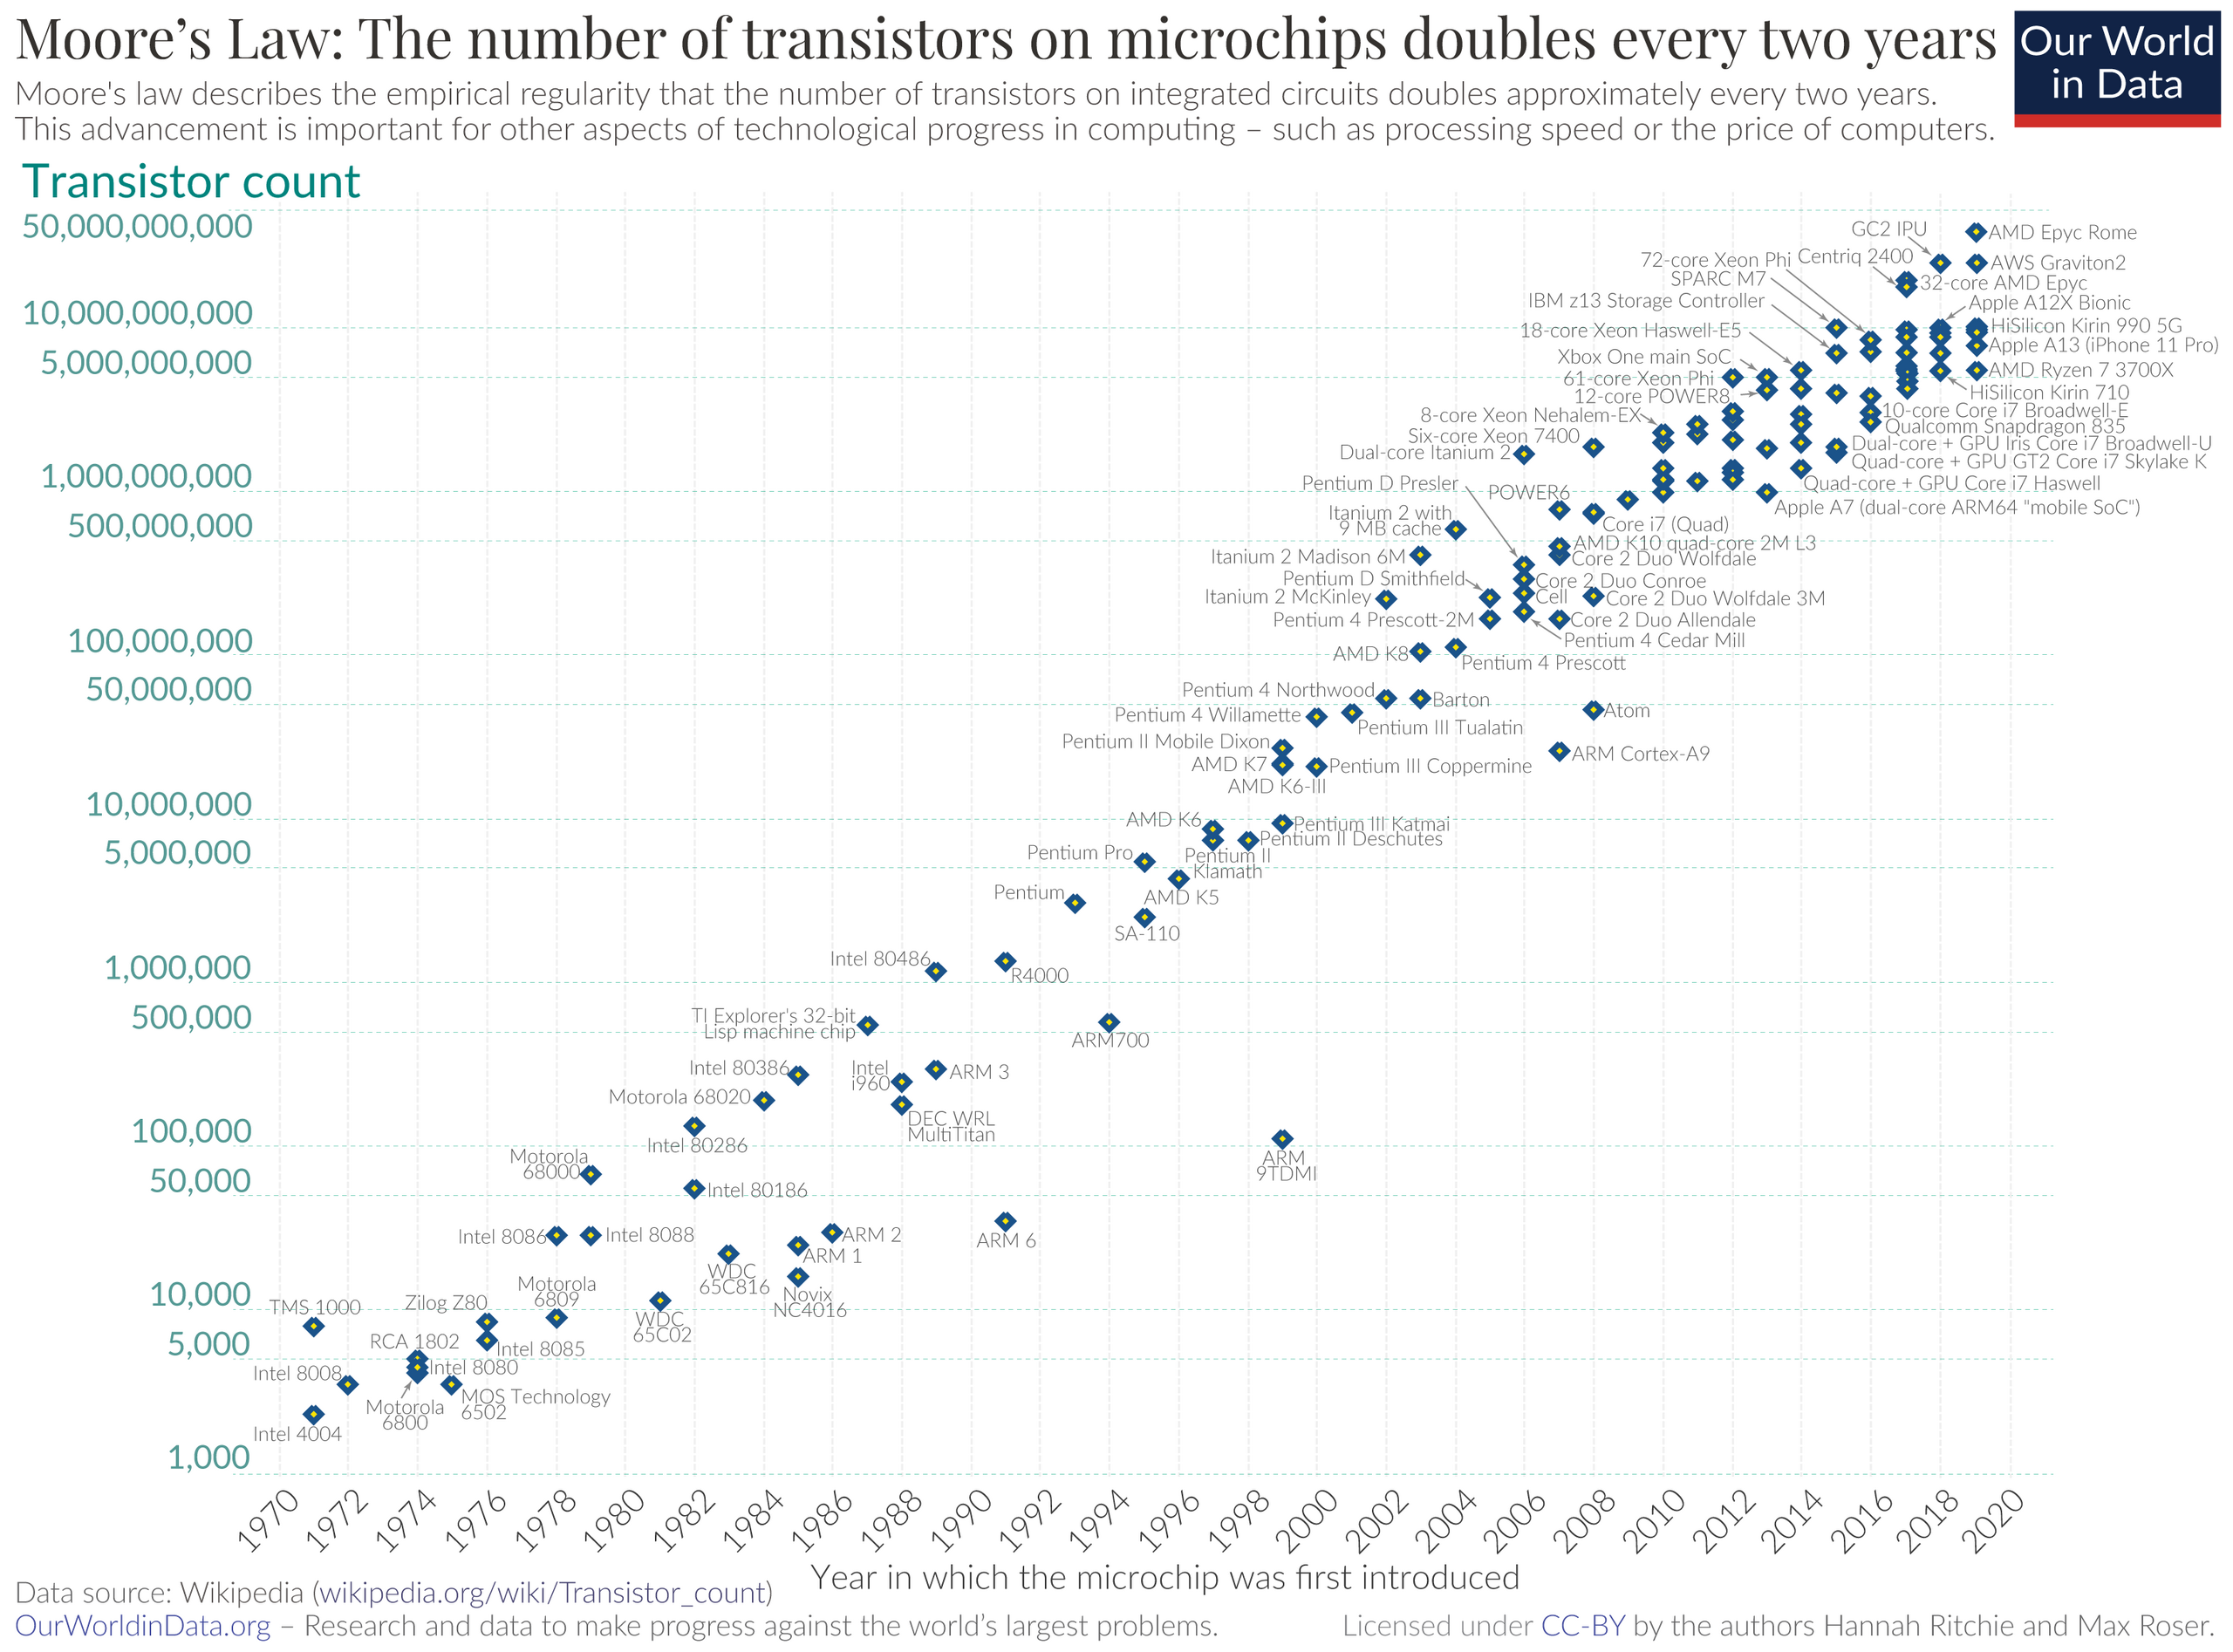
\includegraphics[width=0.6\linewidth]{images/moore.png}
    \caption{Llei de Moore. Gràfic de quantitat de transistors MOS per any. Wikipedia.}
    \label{<label>}
\end{figure}

A continuació, parlarem sobre la història de la tecnologia CMOS, els principis físics, el seu funcionament intern i les seves aplicacions actuals i futures.



\section{Història del CMOS}
% Destacar los hitos importantes desde 1963, comparaciones con tecnologías anteriores (NMOS, BJT).
% Mencionar su adopción masiva en los años 80-90 y cómo ha evolucionado.

\subsection{BJT i MOSFET}

\begin{wrapfigure}{r}{0.25\paperwidth}
    \centering
    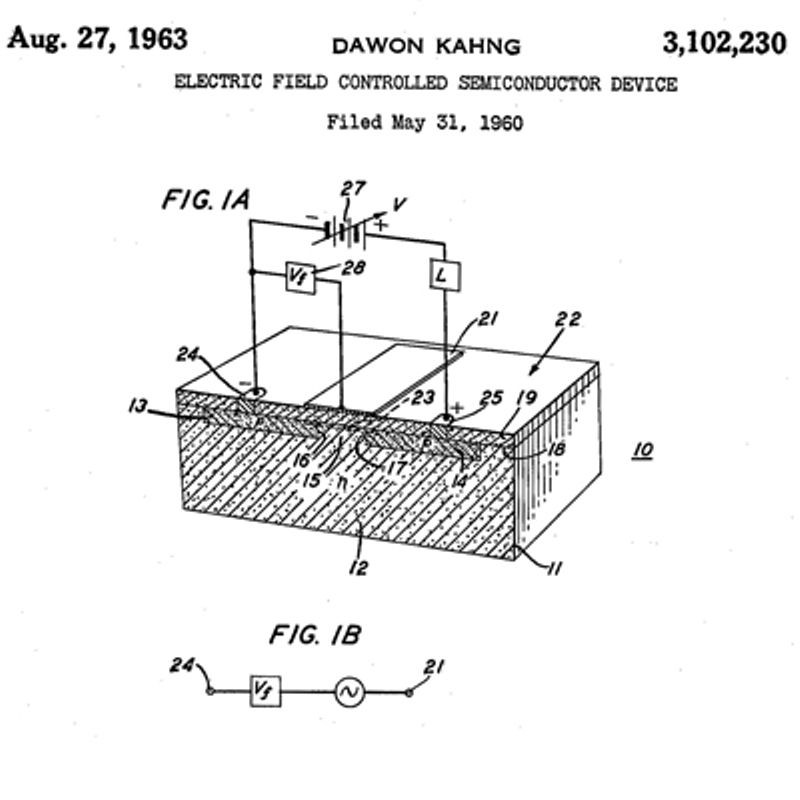
\includegraphics[width=\linewidth]{images/patent kahang.jpg}
    \caption{Patent \texttt{US3102230A} estatunidenca del MOSFET de Dawon Kahng.}
\end{wrapfigure}
Al final dels anys 1940, el transistor bipolar de junció, o BJT, va ser inventat per John Bardeen i Walter Brattain sota la direcció de William Shockley als laboratoris Bell Telephone. Gràcies a certes millores introduïdes de cara a l'eficiència, tant en el seu ús com a la seva producció, van ser introduïts al públic general als principis dels anys 1950 i van ser la tecnologia predominant al mercat durant trenta anys.


Prèviament, el transistor d'efecte de camp semiconductor-òxid-metall, o MOSFET, ja s'havia inventat i patentat a Europa. Aquest va ser objecte d'estudi per part de l'equip dels laboratoris Bell, però sense èxit, a causa dels problemes dels estats superficials \footnote{Els estats superficials són els estats electrònics que es formen a la superfície dels materials, deguts a la interrupció de la malla atòmica del material que acaba en la superfície. Aquest efecte es pot pal$\cdot$liar amb la \textit{passivització} de la superfície, que redueix l'efecte i estabilitza els estats electrònics al límit del material.} no va ser possible la seva adopció a gran escala.

Després d'avenços amb el transistor (òxid de Silici com a passivitzador, invenció de la tecnologia de fabricació planar), finalment Mohamed Atalla i Dawon Kahng van introduir el primer transistor MOS de silici funcional als laboratoris Bell l'any 1960. 

Tot i això, els transistors MOSFET no estaven a l'altura dels BJT de l'època i eren vistos com a inferiors. 

La principal diferència entre els MOSFET i BJT és el consum elèctric i el seu ús típic: 
\begin{itemize}
    \item Els BJT són controlats per corrent a la base, i aquest corrent controla el flux entre el col·lector i l'emissor. Tenen un comportament lineal i són ideals per a circuits analògics. Requereixen un flux de corrent constant per funcionar.
    \item Els MOSFET, quan s'utilitzen en configuració CMOS, només consumeixen energia durant els canvis d'estat (commutació), cosa que els fa especialment adequats per a circuits digitals. Fora de CMOS, generalment PMOS i NMOS per separat, els MOSFET també poden consumir energia de forma contínua segons com estiguin polaritzats.
\end{itemize}

\begin{wrapfigure}{r}{0.2\paperwidth}
    \centering
    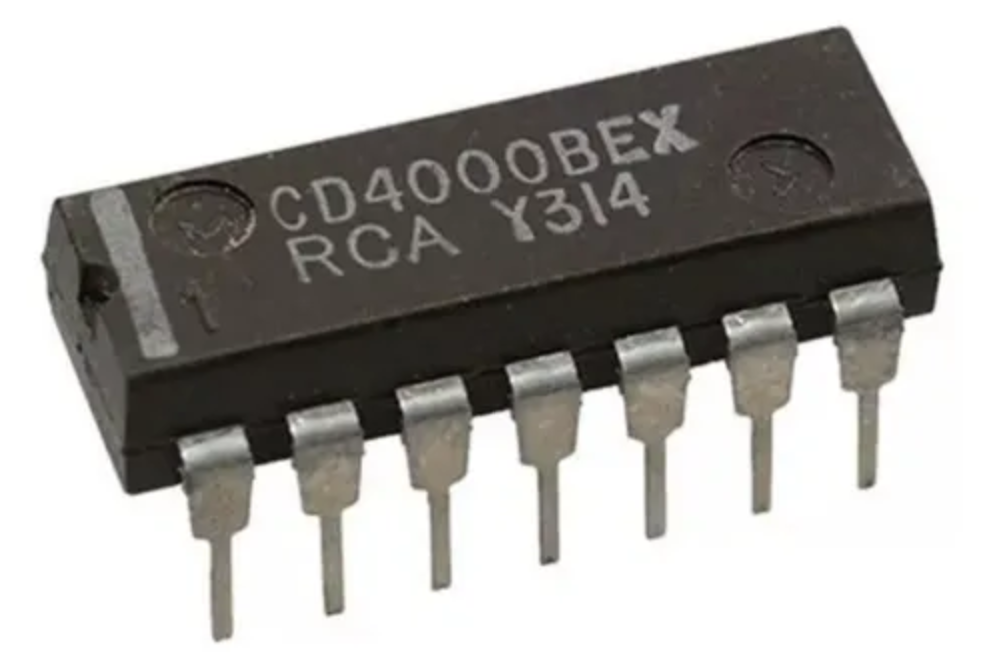
\includegraphics[width=\linewidth]{images/rca cd4000 chip.png}
    \caption{Chip de la familia CD4000 de RCA.}
\end{wrapfigure}
El primer circuit integrat amb tecnologia MOSFET (únicament PMOS) va ser presentat al 1964 per General Microelectronics i el primer aparell d'us quotidià (una calculadora) amb aquests circuits va ser presentada per la mateixa empresa un any després\autocite{general_microelectronics}.


\subsection{Naixement del CMOS, primers dispositius}


El concepte del CMOS neix de reduir el consum energètic dels NMOS i PMOS utilitzats de forma singular i no en conjunt. 

Aquesta tecnologia es presenta al 1960 per la companyia Fairchild Semiconductor però la seva primera comercialització es va prorrogar fins al 1968 amb la presentació del chip CD4000 per RCA\autocite{wiki:4000-series_integrated_circuits}.




\subsection{Actualitat}

\section{Funcionament intern}

\subsection{Estructura d'un CMOS}
% Describir un inversor básico nMOS/pMOS en serie con explicación de entrada/salida.

\subsection{Bandes d'energia}
% Explicar las bandas de valencia/conducción en nMOS y pMOS, con comentario sobre inversión de canal.
% Comentar brevemente el modelo de portadores mayoritarios.

\subsection{Corrent de portadors}
% Diferenciar entre flujo de electrones (nMOS) y huecos (pMOS). 
% Mencionar el principio de conducción dependiente del voltaje de puerta.

% \subsection{Consumo de Potencia}
% % Diferenciar entre consumo estático y dinámico.
% % Comentar sobre la eficiencia del CMOS frente a otras tecnologías.

\section{Aplicacions}

\subsection{Portes lògiques}

\subsection{Sensors i cameres digitals}
% Cámaras digitales, sensores industriales, robótica.

\printbibliography

\end{document}
